\documentclass[]{article}
\usepackage{lmodern}
\usepackage{amssymb,amsmath}
\usepackage{ifxetex,ifluatex}
\usepackage{fixltx2e} % provides \textsubscript
\ifnum 0\ifxetex 1\fi\ifluatex 1\fi=0 % if pdftex
  \usepackage[T1]{fontenc}
  \usepackage[utf8]{inputenc}
\else % if luatex or xelatex
  \ifxetex
    \usepackage{mathspec}
  \else
    \usepackage{fontspec}
  \fi
  \defaultfontfeatures{Ligatures=TeX,Scale=MatchLowercase}
\fi
% use upquote if available, for straight quotes in verbatim environments
\IfFileExists{upquote.sty}{\usepackage{upquote}}{}
% use microtype if available
\IfFileExists{microtype.sty}{%
\usepackage{microtype}
\UseMicrotypeSet[protrusion]{basicmath} % disable protrusion for tt fonts
}{}
\usepackage[margin=1in]{geometry}
\usepackage{hyperref}
\hypersetup{unicode=true,
            pdftitle={MATH 530/630},
            pdfborder={0 0 0},
            breaklinks=true}
\urlstyle{same}  % don't use monospace font for urls
\usepackage{color}
\usepackage{fancyvrb}
\newcommand{\VerbBar}{|}
\newcommand{\VERB}{\Verb[commandchars=\\\{\}]}
\DefineVerbatimEnvironment{Highlighting}{Verbatim}{commandchars=\\\{\}}
% Add ',fontsize=\small' for more characters per line
\usepackage{framed}
\definecolor{shadecolor}{RGB}{248,248,248}
\newenvironment{Shaded}{\begin{snugshade}}{\end{snugshade}}
\newcommand{\KeywordTok}[1]{\textcolor[rgb]{0.13,0.29,0.53}{\textbf{#1}}}
\newcommand{\DataTypeTok}[1]{\textcolor[rgb]{0.13,0.29,0.53}{#1}}
\newcommand{\DecValTok}[1]{\textcolor[rgb]{0.00,0.00,0.81}{#1}}
\newcommand{\BaseNTok}[1]{\textcolor[rgb]{0.00,0.00,0.81}{#1}}
\newcommand{\FloatTok}[1]{\textcolor[rgb]{0.00,0.00,0.81}{#1}}
\newcommand{\ConstantTok}[1]{\textcolor[rgb]{0.00,0.00,0.00}{#1}}
\newcommand{\CharTok}[1]{\textcolor[rgb]{0.31,0.60,0.02}{#1}}
\newcommand{\SpecialCharTok}[1]{\textcolor[rgb]{0.00,0.00,0.00}{#1}}
\newcommand{\StringTok}[1]{\textcolor[rgb]{0.31,0.60,0.02}{#1}}
\newcommand{\VerbatimStringTok}[1]{\textcolor[rgb]{0.31,0.60,0.02}{#1}}
\newcommand{\SpecialStringTok}[1]{\textcolor[rgb]{0.31,0.60,0.02}{#1}}
\newcommand{\ImportTok}[1]{#1}
\newcommand{\CommentTok}[1]{\textcolor[rgb]{0.56,0.35,0.01}{\textit{#1}}}
\newcommand{\DocumentationTok}[1]{\textcolor[rgb]{0.56,0.35,0.01}{\textbf{\textit{#1}}}}
\newcommand{\AnnotationTok}[1]{\textcolor[rgb]{0.56,0.35,0.01}{\textbf{\textit{#1}}}}
\newcommand{\CommentVarTok}[1]{\textcolor[rgb]{0.56,0.35,0.01}{\textbf{\textit{#1}}}}
\newcommand{\OtherTok}[1]{\textcolor[rgb]{0.56,0.35,0.01}{#1}}
\newcommand{\FunctionTok}[1]{\textcolor[rgb]{0.00,0.00,0.00}{#1}}
\newcommand{\VariableTok}[1]{\textcolor[rgb]{0.00,0.00,0.00}{#1}}
\newcommand{\ControlFlowTok}[1]{\textcolor[rgb]{0.13,0.29,0.53}{\textbf{#1}}}
\newcommand{\OperatorTok}[1]{\textcolor[rgb]{0.81,0.36,0.00}{\textbf{#1}}}
\newcommand{\BuiltInTok}[1]{#1}
\newcommand{\ExtensionTok}[1]{#1}
\newcommand{\PreprocessorTok}[1]{\textcolor[rgb]{0.56,0.35,0.01}{\textit{#1}}}
\newcommand{\AttributeTok}[1]{\textcolor[rgb]{0.77,0.63,0.00}{#1}}
\newcommand{\RegionMarkerTok}[1]{#1}
\newcommand{\InformationTok}[1]{\textcolor[rgb]{0.56,0.35,0.01}{\textbf{\textit{#1}}}}
\newcommand{\WarningTok}[1]{\textcolor[rgb]{0.56,0.35,0.01}{\textbf{\textit{#1}}}}
\newcommand{\AlertTok}[1]{\textcolor[rgb]{0.94,0.16,0.16}{#1}}
\newcommand{\ErrorTok}[1]{\textcolor[rgb]{0.64,0.00,0.00}{\textbf{#1}}}
\newcommand{\NormalTok}[1]{#1}
\usepackage{graphicx,grffile}
\makeatletter
\def\maxwidth{\ifdim\Gin@nat@width>\linewidth\linewidth\else\Gin@nat@width\fi}
\def\maxheight{\ifdim\Gin@nat@height>\textheight\textheight\else\Gin@nat@height\fi}
\makeatother
% Scale images if necessary, so that they will not overflow the page
% margins by default, and it is still possible to overwrite the defaults
% using explicit options in \includegraphics[width, height, ...]{}
\setkeys{Gin}{width=\maxwidth,height=\maxheight,keepaspectratio}
\IfFileExists{parskip.sty}{%
\usepackage{parskip}
}{% else
\setlength{\parindent}{0pt}
\setlength{\parskip}{6pt plus 2pt minus 1pt}
}
\setlength{\emergencystretch}{3em}  % prevent overfull lines
\providecommand{\tightlist}{%
  \setlength{\itemsep}{0pt}\setlength{\parskip}{0pt}}
\setcounter{secnumdepth}{0}
% Redefines (sub)paragraphs to behave more like sections
\ifx\paragraph\undefined\else
\let\oldparagraph\paragraph
\renewcommand{\paragraph}[1]{\oldparagraph{#1}\mbox{}}
\fi
\ifx\subparagraph\undefined\else
\let\oldsubparagraph\subparagraph
\renewcommand{\subparagraph}[1]{\oldsubparagraph{#1}\mbox{}}
\fi

%%% Use protect on footnotes to avoid problems with footnotes in titles
\let\rmarkdownfootnote\footnote%
\def\footnote{\protect\rmarkdownfootnote}

%%% Change title format to be more compact
\usepackage{titling}

% Create subtitle command for use in maketitle
\newcommand{\subtitle}[1]{
  \posttitle{
    \begin{center}\large#1\end{center}
    }
}

\setlength{\droptitle}{-2em}

  \title{MATH 530/630}
    \pretitle{\vspace{\droptitle}\centering\huge}
  \posttitle{\par}
  \subtitle{Integrative Lab 3}
  \author{}
    \preauthor{}\postauthor{}
    \date{}
    \predate{}\postdate{}
  

\begin{document}
\maketitle

{
\setcounter{tocdepth}{2}
\tableofcontents
}
\section{Overview}\label{overview}

The goal of this lab is to carefully, thoroughly, and thoughtfully
compare two group means and understand the results. You are also asked
to communicate clearly about the steps in your analysis process with
others, by sharing your R code, output, and narrative. As such, your
code cannot ``stand alone''- it is meant to complement / enhance /
support your narrative. As with our previous
\href{cm026.html}{integrative lab}, this lab will be due in two stages:

\begin{enumerate}
\def\labelenumi{\arabic{enumi}.}
\tightlist
\item
  A complete knitted \texttt{html} file is due on Sakai by Thursday
  August 30th at 2:30pm.
\item
  After class on August 30th, you'll be provided with a code key. You
  are asked to review your initial submission, and reflect on your own
  code/narrative after reviewing the key thoroughly. Your
  self-assessment is due on Sakai by beginning of class Thursday
  September 6th (2:30pm).
\end{enumerate}

Using the key, your self-assessment should include even \textbf{more}
narrative; where you made mistakes, you must discuss and analyze where
you went wrong, and correct them without copying/pasting directly from
the key (this typically means that you need to include more narrative
than we provide in the key). A good self-assessment will include:

\begin{itemize}
\tightlist
\item
  Assessment of the accuracy and completeness of your ``initial
  solutions''
\item
  Correct worked solutions with some discussion and analysis of why your
  initial solution was incorrect, and reflection on the source of your
  confusion (if you got an answer correct, this is not necessary)
\item
  Attributions as appropriate to other students who helped you, or other
  sources such as lecture notes, readings, online resources, etc. that
  helped you
\end{itemize}

\section{Headnotes}\label{headnotes}

\begin{itemize}
\tightlist
\item
  This lab is based on the assigned reading that includes
  \href{http://moderndive.netlify.com/10-hypothesis-testing.html\#theory-hypo}{ModernDive
  Chapter 10.8 on t-tests for comparing two independent samples}. Please
  open and follow closely!
\item
  Also see \href{http://moderndive.netlify.com/b-appendixb}{ModernDive
  Appendix B} for examples (search for:
  \texttt{B.5.5\ Traditional\ methods})
\item
  Parts of this lab are adapted from Ted Laderas' and Jessica Minnier's
  \href{https://www.datacamp.com/courses/rbootcamp}{R Bootcamp} on
  DataCamp.com
\end{itemize}

\section{Packages}\label{packages}

Please install a new version of \texttt{infer} first:

\begin{Shaded}
\begin{Highlighting}[]
\NormalTok{remotes}\OperatorTok{::}\KeywordTok{install_github}\NormalTok{(}\StringTok{"tidymodels/infer"}\NormalTok{, }\DataTypeTok{ref =} \StringTok{"develop"}\NormalTok{)}
\end{Highlighting}
\end{Shaded}

\begin{Shaded}
\begin{Highlighting}[]
\KeywordTok{library}\NormalTok{(tidyverse)}
\KeywordTok{library}\NormalTok{(infer)}
\KeywordTok{library}\NormalTok{(skimr)}
\KeywordTok{library}\NormalTok{(broom)}
\end{Highlighting}
\end{Shaded}

\section{Data}\label{data}

We are going to work with a dataset called
\href{https://raw.githubusercontent.com/apreshill/ohsu-basic-stats/master/data/fishermen_mercury.csv}{\texttt{fishermen\_mercury.csv}},
which consists of factors related to mercury levels among fishermen and
a control group of non-fishermen. The data are published within the
paper available
\href{https://www.sciencedirect.com/science/article/pii/S0269749199002614?via\%3Dihub\#TBL2}{online}.
Here is the citation for the peer-reviewed publication:

\begin{quote}
N.B. Al-Majed and M.R. Preston (2000). ``Factors Influencing the Total
Mercury and Methyl Mercury in the Hair of Fishermen in Kuwait,''
Environmental Pollution, Vol. 109, pp.~239-250.
\end{quote}

\begin{verbatim}
Error in .f(.x[[i]], ...): object 'TotHg' not found
\end{verbatim}

\begin{verbatim}
Error in is.data.frame(x): object 'mercury' not found
\end{verbatim}

\begin{Shaded}
\begin{Highlighting}[]
\NormalTok{mercury <-}\StringTok{ }\KeywordTok{read_csv}\NormalTok{(here}\OperatorTok{::}\KeywordTok{here}\NormalTok{(}\StringTok{"data"}\NormalTok{, }\StringTok{"fishermen_mercury.csv"}\NormalTok{),}
                    \DataTypeTok{col_types =} \KeywordTok{cols}\NormalTok{(}
                      \DataTypeTok{fisherman =} \KeywordTok{col_factor}\NormalTok{(}\DataTypeTok{levels =} \OtherTok{NULL}\NormalTok{))}
\NormalTok{                    )}
\end{Highlighting}
\end{Shaded}

Variables in this dataset include:

\begin{itemize}
\tightlist
\item
  Fisherman indicator (\texttt{fisherman})
\item
  Age in years (\texttt{age})
\item
  Residence Time in years (\texttt{restime})
\item
  Height in cm (\texttt{height})
\item
  Weight in kg (\texttt{weight})
\item
  Fish meals per week (\texttt{fishmlwk})
\item
  Parts of fish consumed:

  \begin{itemize}
  \tightlist
  \item
    0=none,
  \item
    1=muscle tissue only,
  \item
    2=mt and sometimes whole fish,
  \item
    3=whole fish (fishpart)
  \end{itemize}
\item
  Methyl Mercury in mg/g (\texttt{methyl\_mercury})
\item
  Total Mercury in mg/g (\texttt{total\_mercury})
\end{itemize}

\section{Motivating research
question}\label{motivating-research-question}

Do fishermen have different levels of total mercury than non-fishermen?

\section{Exploratory data analysis}\label{exploratory-data-analysis}

Explore the \texttt{fisherman} and \texttt{total\_mercury} variables.
Recall that a
\href{http://moderndive.netlify.com/6-regression.html\#model1EDA}{new
exploratory data analysis} involves three things:

\begin{itemize}
\tightlist
\item
  Looking at the raw values.
\item
  Computing summary statistics of the variables of interest.
\item
  Creating informative visualizations.
\end{itemize}

General functions that we have used at this stage:

\begin{itemize}
\tightlist
\item
  \texttt{dplyr::glimpse()}
\item
  \texttt{skimr::skim()}

  \begin{itemize}
  \tightlist
  \item
    Given the two-group design, you may wish to do a
    \texttt{dplyr::group\_by()} first here
  \end{itemize}
\item
  \texttt{ggplot2::ggplot()}

  \begin{itemize}
  \tightlist
  \item
    \texttt{geom\_histogram()} or \texttt{geom\_density()} or
    \texttt{geom\_boxplot()} for numeric continuous variables

    \begin{itemize}
    \tightlist
    \item
      Given the two-group design, you may wish to combine these with
      \texttt{facet\_wrap()}
    \end{itemize}
  \item
    \texttt{geom\_bar()} or \texttt{geom\_col()} for categorical
    variables
  \end{itemize}
\end{itemize}

You may also find your want to use \texttt{filter}, \texttt{mutate},
\texttt{arrange}, \texttt{select}, or \texttt{count}. Let your questions
lead you!

\section{Check conditions}\label{check-conditions}

Remember that in order to use the short-cut (formula-based, theoretical)
approach, we need to check that some conditions are met. The
\texttt{infer} package does not automatically check conditions for the
theoretical methods to work. In order for the results of the \(t\)-test
to be valid, three conditions must be met:

\begin{enumerate}
\def\labelenumi{\arabic{enumi}.}
\tightlist
\item
  Independent observations in both samples
\item
  Nearly normal populations OR large sample sizes (\(n \ge 30\))
\item
  Independently selected samples
\item
  For this lab, we'll also assume that the variance in the
  response/outcome variable is \emph{the same} for both groups
\end{enumerate}

Write a few sentences to address each of these conditions.

\section{\texorpdfstring{\(t\)-test for two independent
samples}{t-test for two independent samples}}\label{t-test-for-two-independent-samples}

The following are excerpts from ModernDive:

\begin{quote}
``The most common normalization is known as the \(z\)-score. The formula
for a \(z\)-score is \[Z = \frac{x - \mu}{\sigma},\] where \(x\)
represent the value of a variable, \(\mu\) represents the mean of the
variable, and \(\sigma\) represents the standard deviation of the
variable. Thus, if your variable has 10 elements, each one has a
corresponding \(z\)-score that gives how many standard deviations away
that value is from its mean. \(z\)-scores are normally distributed with
mean 0 and standard deviation 1. They have the common, bell-shaped
pattern seen below.''
\end{quote}

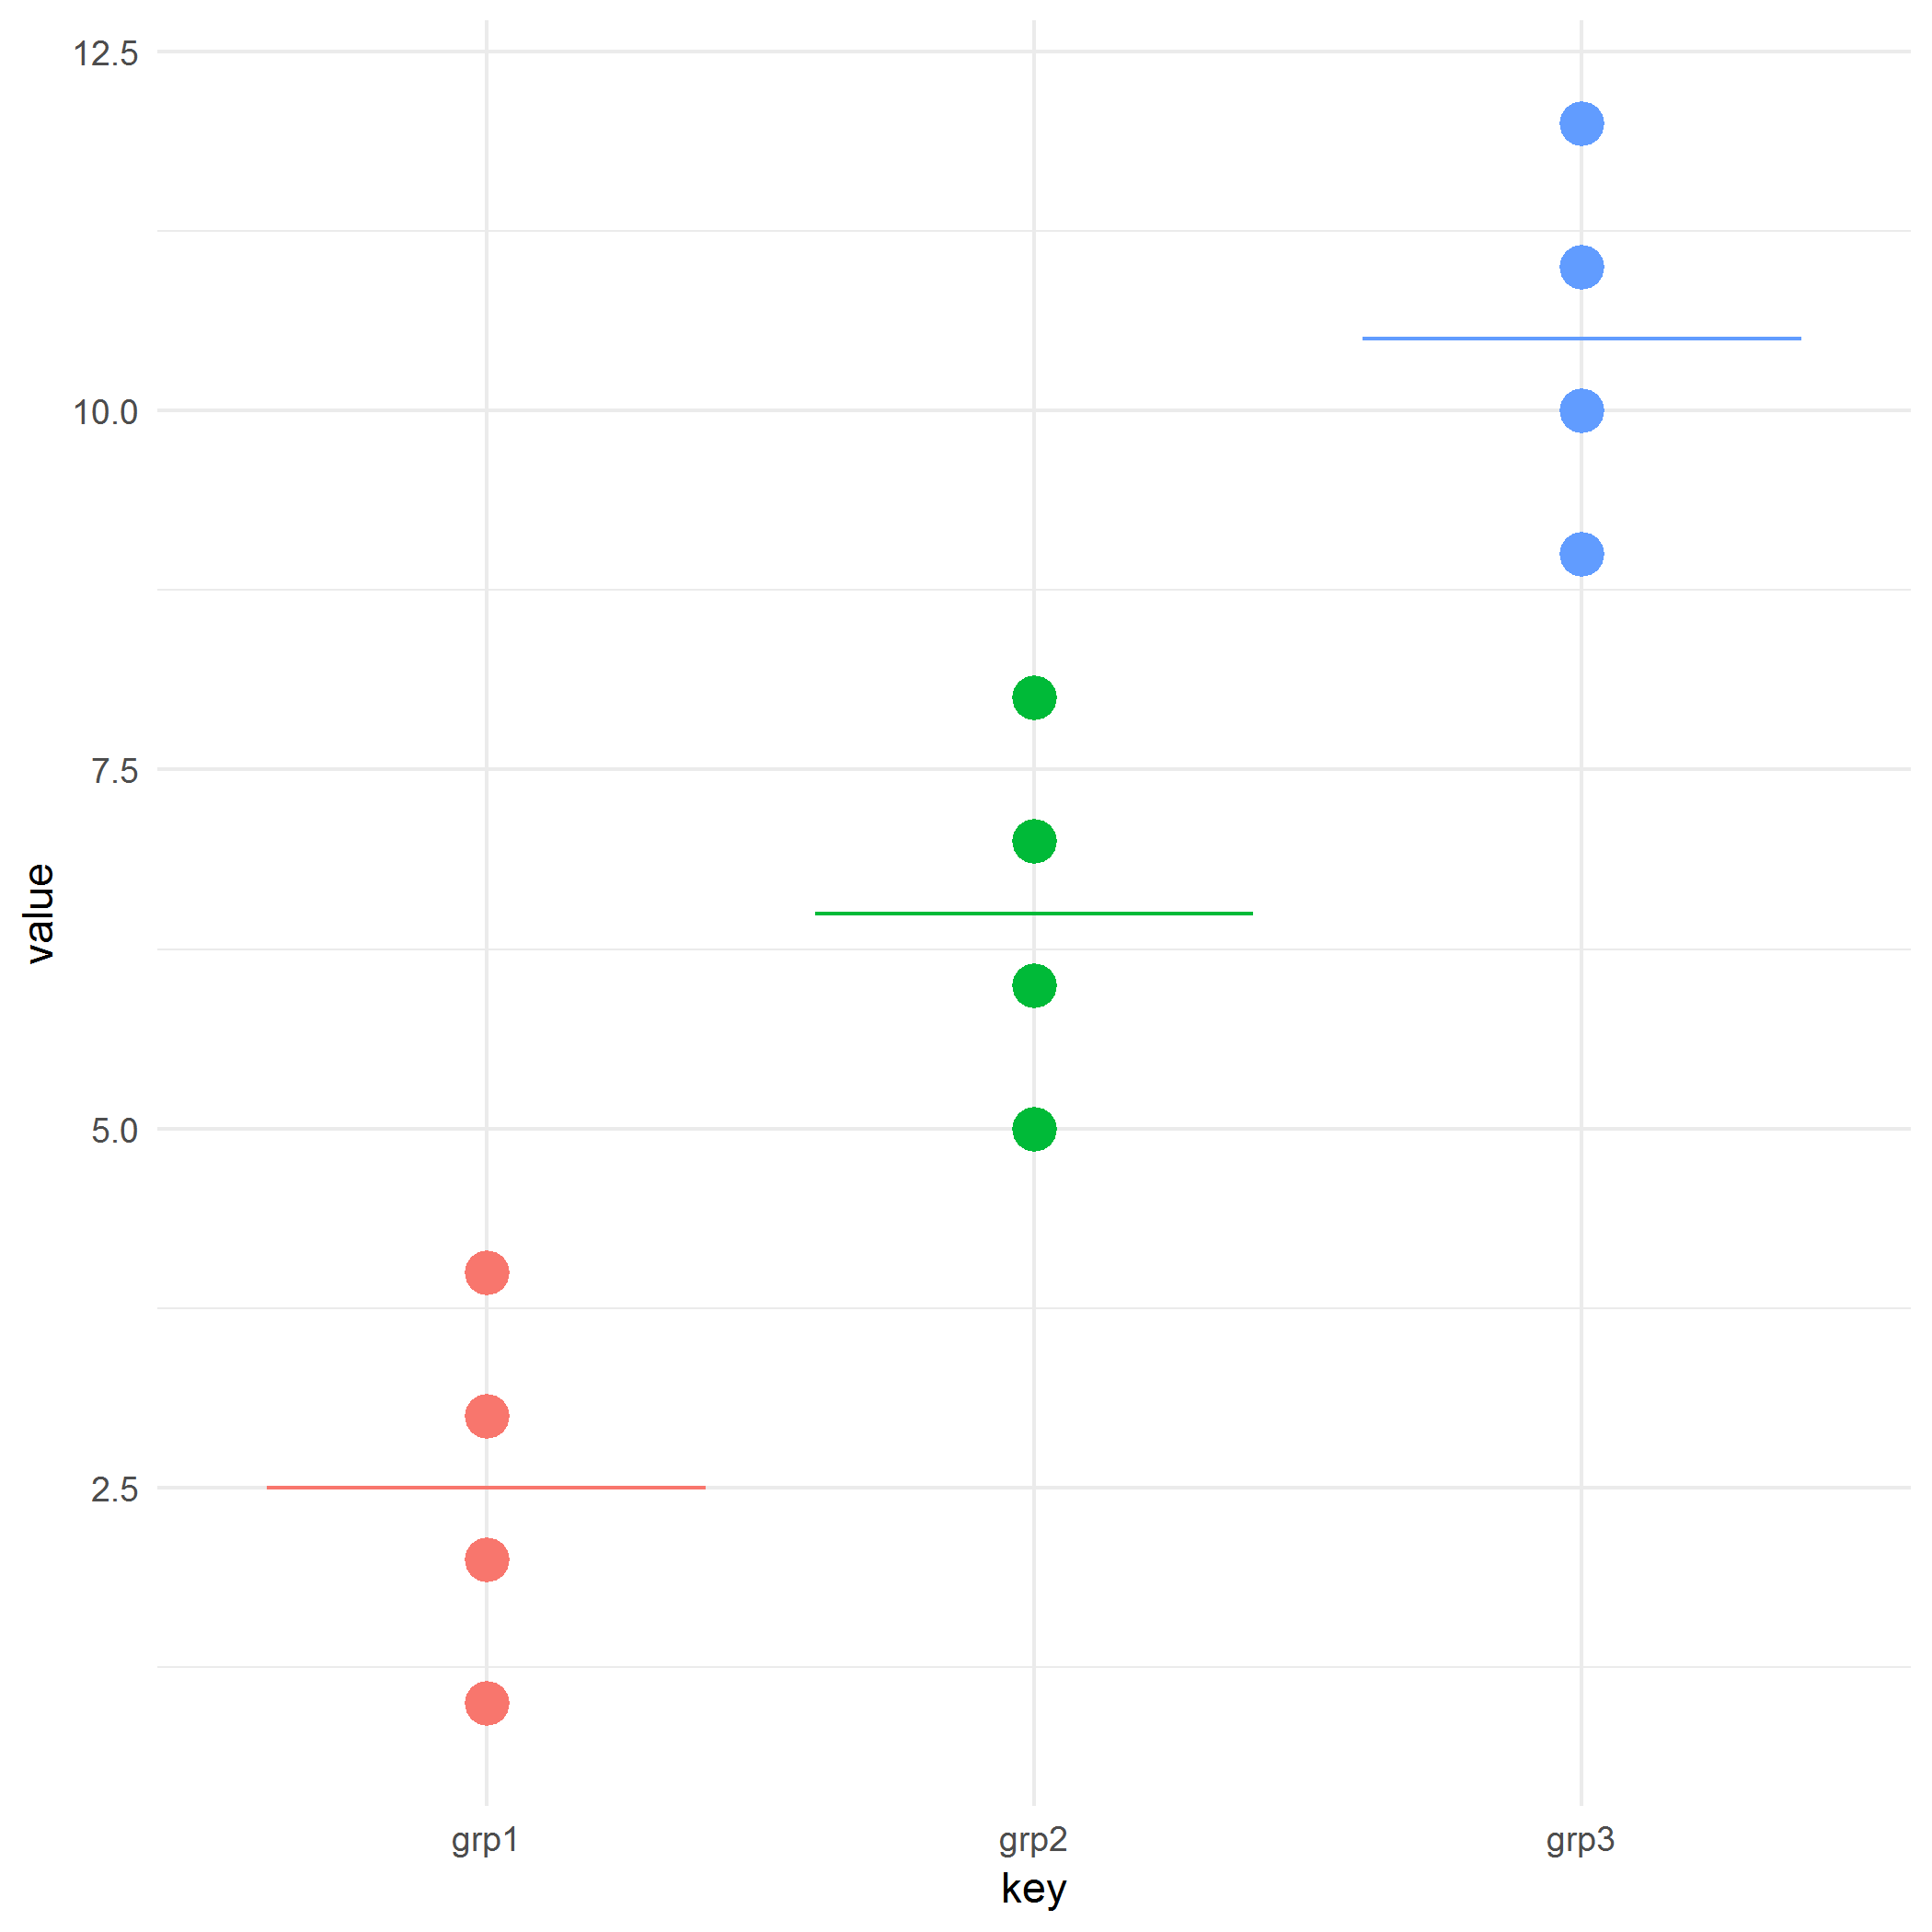
\includegraphics{lab03_files/figure-latex/unnamed-chunk-6-1.pdf}

\begin{quote}
``Recall, that we hardly ever know the mean and standard deviation of
the population of interest. This is almost always the case when
considering the means of two independent groups. To help account for us
not knowing the population parameter values, we can use the sample
statistics instead, but this comes with a bit of a price in terms of
complexity.''
\end{quote}

\subsection{\texorpdfstring{Test statistic
\(\delta\)}{Test statistic \textbackslash{}delta}}\label{test-statistic-delta}

\begin{quote}
``Another form of normalization occurs when we need to use the sample
standard deviations as estimates for the unknown population standard
deviations. This normalization is often called the \(t\)-score.''
\end{quote}

For the two independent samples case like what we have for comparing
fishermen to non-fishermen, the formula is
\[{\displaystyle T={\frac {({\bar {x}}_{1}-{\bar {x}}_{2})- (\mu_1-\mu_2)}{s_{p}\times {\sqrt {{\frac {1}{n_{1}}}+{\frac {1}{n_{2}}}}}}}}\]

where\ldots{}

\begin{itemize}
\tightlist
\item
  \(\bar{x}_1\) is the sample mean response of the first group
\item
  \(\bar{x}_2\) is the sample mean response of the second group
\item
  \(\mu_1\) is the population mean response of the first group
\item
  \(\mu_2\) is the population mean response of the second group
\item
  \(s_p\) is the pooled standard deviation of the two samples
\item
  The overall denominator is called the standard error of the difference
  between means.
\end{itemize}

From the
\href{http://blog.minitab.com/blog/adventures-in-statistics-2/understanding-t-tests-t-values-and-t-distributions}{Minitab
blog}:

\begin{quote}
``A t-value of 0 indicates that the sample results exactly equal the
null hypothesis. As the difference between the sample data and the null
hypothesis increases, the absolute value of the t-value increases.''
\end{quote}

Note that the quantity \((\mu_1 - \mu_2)\) is typically 0 under the null
hypothesis, so the actual computational formula for the \(t\)-statistic
is:

\[{\displaystyle T={\frac {{\bar {x}}_{1}-{\bar {x}}_{2}}{s_{p}\times {\sqrt {{\frac {1}{n_{1}}}+{\frac {1}{n_{2}}}}}}}}\]

where\ldots{}

\[{\displaystyle s_{p}=
{\sqrt {\frac {\left(n_{1}-1\right)s_{1}^{2}+\left(n_{2}-1\right)s_{2}^{2}}{n_{1}+n_{2}-2}}}}\]

where\ldots{}

\begin{itemize}
\tightlist
\item
  \(s_1\) is the sample standard deviation of the response of the first
  group
\item
  \(s_2\) is the sample standard deviation of the response of the second
  group
\item
  \(n_1\) is the sample size of the first group
\item
  \(n_2\) is the sample size of the second group
\end{itemize}

The \(s_p\) here is called the ``pooled standard deviation.'' Now that
we have two samples (in our case, fishermen and non-fishermen), we have
two standard deviations. Recall that in order to calculate the standard
error of one mean we divided the sample standard deviation by the square
root of \(N\). The pooled standard error is the same idea, but after
combining the standard deviations from two samples. The calculation is
important, as it assumes that \emph{there is not a difference} in the
standard deviations between the two groups, and hence they can be
pooled. Remember that \(s^2\) is the squared standard deviation, which
we know is the variance (i.e., \texttt{var(x1)} = \texttt{(sd(x1))\^{}2}
and \texttt{sd(x1)} = \texttt{sqrt(var(x1))}).

Given the above formulas, answer the following questions using R code
plus narrative:

\begin{itemize}
\item
  What is the pooled standard error for the \texttt{total\_mercury}
  variable? (try to make all quantities here defined variables using
  \texttt{dplyr::group\_by()\ \%\textgreater{}\%\ summarize()\ \%\textgreater{}\%\ filter()\ \%\textgreater{}\%\ pull()})
\item
  What are the minimum \(t\)-statistic values we need to conclude that
  there is a significant difference at \(\alpha = .05\) (2-tailed)?
  (hint: degrees of freedom for a two-sample t-test are \(N\) - 2)
\item
  Use the following code to plot these critical t-values.
\end{itemize}

\begin{Shaded}
\begin{Highlighting}[]
\NormalTok{upper_tcrit <-}\StringTok{ }\CommentTok{# fill in here}
\NormalTok{mercury }\OperatorTok\StringTok{ }
\StringTok{  }\KeywordTok{specify}\NormalTok{(total_mercury }\OperatorTok{~}\StringTok{ }\NormalTok{fisherman) }\OperatorTok\StringTok{ }
\StringTok{  }\KeywordTok{hypothesize}\NormalTok{(}\DataTypeTok{null =} \StringTok{"independence"}\NormalTok{) }\OperatorTok\StringTok{ }
\StringTok{  }\KeywordTok{calculate}\NormalTok{(}\DataTypeTok{stat =} \StringTok{"t"}\NormalTok{, }\DataTypeTok{order =} \KeywordTok{c}\NormalTok{(}\DecValTok{1}\NormalTok{,}\DecValTok{0}\NormalTok{)) }\OperatorTok
\StringTok{  }\KeywordTok{visualize}\NormalTok{(}\DataTypeTok{method =} \StringTok{"theoretical"}\NormalTok{, }
            \DataTypeTok{obs_stat =}\NormalTok{ upper_tcrit, }
            \DataTypeTok{direction =} \StringTok{"both"}\NormalTok{) }\CommentTok{# gives us shading}
\end{Highlighting}
\end{Shaded}

\begin{itemize}
\tightlist
\item
  Now we know the minimum \(t\)-statistic value we need to beat, what is
  the minimum absolute value for the mean difference we need to detect
  significance with \(\alpha = .05\) (2-tailed)? (big hint: realize that
  the rearranged formula below may be helpful!)
\end{itemize}

\[{\displaystyle T \times {s_{p}\times {\sqrt {{\frac {1}{n_{1}}}+{\frac {1}{n_{2}}}}}}}={{\bar {x}}_{1}-{\bar {x}}_{2}}\]

\begin{itemize}
\tightlist
\item
  Complete this sentence filling in numbers from your above
  calculations:
\end{itemize}

\begin{quote}
With \(n_1\) fisherman and \(n_2\) non-fishermen, given the variability
in total mercury present in this sample, we will reject the null
hypothesis that there is no difference in total mercury levels between
the two groups if we obtain a \(t\)-statistic greater than X (absolute
value, \(\alpha\) = .05, 2-tailed). This is equivalent to saying we will
reject the null hypothesis if we obtain a mean difference greater than X
(absolute value, \(\alpha\) = .05, 2-tailed).
\end{quote}

\subsection{\texorpdfstring{Observed effect
\(\delta^*\)}{Observed effect \textbackslash{}delta\^{}*}}\label{observed-effect-delta}

Answer the following questions using R code and narrative:

\begin{itemize}
\item
  What mean difference (raw) did we observe? Is it greater than the
  minimum mean difference we need to beat? (hint: try
  \texttt{infer::specify} then \texttt{calculate} with
  \texttt{stat\ =\ "diff\ in\ means"}).
\item
  Calculate the \(t\)-statistic ``by hand'' using R. Is it greater than
  the minimum \(t\)-statistic we need to beat? (here is the formula
  again):
\end{itemize}

\[{\displaystyle T={\frac {{\bar {x}}_{1}-{\bar {x}}_{2}}{s_{p}\times {\sqrt {{\frac {1}{n_{1}}}+{\frac {1}{n_{2}}}}}}}}\]

\begin{itemize}
\tightlist
\item
  Do a classical 2-sample t-test (assuming equal variances, more on this
  later) in R using \texttt{infer}, do the results match your
  calculations?:
\end{itemize}

\begin{Shaded}
\begin{Highlighting}[]
\NormalTok{mercury }\OperatorTok\StringTok{ }
\StringTok{  }\KeywordTok{t_test}\NormalTok{(total_mercury }\OperatorTok{~}\StringTok{ }\NormalTok{fisherman, }\DataTypeTok{order =} \KeywordTok{c}\NormalTok{(}\DecValTok{1}\NormalTok{, }\DecValTok{0}\NormalTok{), }\DataTypeTok{var.equal =} \OtherTok{TRUE}\NormalTok{)}
\end{Highlighting}
\end{Shaded}

\begin{itemize}
\item
  Interpret this output. What is the statistic? What is the
  meaning/interpretation of the confidence interval here? (hint: Does it
  include zero? What does it mean if it does or does not? What value is
  in the center of the interval?)
\item
  Use the code below to compare the normal distribution to the
  \(t\)-distribution, which has only one parameter: degrees of freedom
  (\texttt{df}). You can use the \texttt{dt} and \texttt{dnorm} with the
  \texttt{stat\_function} layer in \texttt{ggplot} to plot the
  \emph{densities} for each distribution. Change the \texttt{df}
  argument here a few times to view its effect: what do you see? (you
  don't need to print any of these plots to your final file- I want you
  to reflect on how the two distributions differ).
\end{itemize}

\begin{Shaded}
\begin{Highlighting}[]
\NormalTok{df <-}\StringTok{ }\DecValTok{10}
\KeywordTok{ggplot}\NormalTok{(}\KeywordTok{data.frame}\NormalTok{(}\DataTypeTok{x =} \KeywordTok{c}\NormalTok{(}\OperatorTok{-}\DecValTok{4}\NormalTok{, }\DecValTok{4}\NormalTok{)), }\KeywordTok{aes}\NormalTok{(x)) }\OperatorTok{+}\StringTok{ }
\StringTok{  }\KeywordTok{stat_function}\NormalTok{(}\DataTypeTok{fun =}\NormalTok{ dt, }\DataTypeTok{args =} \KeywordTok{list}\NormalTok{(}\DataTypeTok{df =}\NormalTok{ df)) }\OperatorTok{+}\StringTok{ }\CommentTok{# t dist}
\StringTok{  }\KeywordTok{stat_function}\NormalTok{(}\DataTypeTok{fun =}\NormalTok{ dnorm, }\DataTypeTok{lty =} \DecValTok{3}\NormalTok{, }\DataTypeTok{color =} \StringTok{"red"}\NormalTok{) }\CommentTok{# normal dist in red}
\end{Highlighting}
\end{Shaded}

\begin{itemize}
\tightlist
\item
  Save your observed \(t\)-statistic, and use \texttt{infer} to make a
  plot of the null t-distribution with a red line for your
  \texttt{obs\_stat}, shading in both directions. Try adding
  \texttt{geom\_vline()} to this object so you can add vertical lines
  where your two ``critical t-values'' are.
\end{itemize}

\subsection{The theoretical p-value}\label{the-theoretical-p-value}

But, how can we calculate the p-value from this? Well the easy way is
with your \texttt{infer} output :) But! Remember that your observed
\(t\)-statistic is a \emph{quantile} value for a statistic that we
\emph{assume} follows a \(t\)-distribution. How do we calculate the
probability of getting a \(t\)-statistic as or more extreme than the one
we got? We use \texttt{pt()}!

\begin{itemize}
\tightlist
\item
  Use \texttt{pt()} to calculate the 2-sided p-value in R. Does it match
  the output from \texttt{infer}?
\end{itemize}

\subsection{The theoretical confidence
interval}\label{the-theoretical-confidence-interval}

Unfortunately, we currently can't get the confidence interval for
theoretical methods using \texttt{infer}. But we can use formulas (yay):

\[ ({\bar {x}}_{1}-{\bar {x}}_{2}) \pm (t_{\star} \times SE_{{\bar {x}}_{1}-{\bar {x}}_{2}})\]
where\ldots{}

\[SE_{{\bar {x}}_{1}-{\bar {x}}_{2}} = s_{p} \times \sqrt {{\frac {1}{n_{1}}}+{\frac {1}{n_{2}}}}\]
You should already have variables for the mean difference and the
\(t\)-statistic critical value(s) (here, \(t_{\star}\)) from the top
formula. In the bottom formula, that standard error should look
familiar- it is the standard error of the difference between means. This
was the denominator in your calculated \(t\)-statistic.

\begin{itemize}
\tightlist
\item
  Use these values to calculate the 95\% confidence interval for the
  difference in means. Does it match the output from \texttt{infer}?
  Does it contain zero? Will this interval ever \emph{not} contain the
  observed difference in sample means?
\end{itemize}

\section{Compare t-test results to permutation
test}\label{compare-t-test-results-to-permutation-test}

Using
\href{http://moderndive.netlify.com/10-hypothesis-testing.html\#example-comparing-two-means}{ModernDive
10.7} as an example, as well as our previous
\href{https://apreshill.github.io/ohsu-basic-stats/cm034.html}{resampling
lab}, conduct a permutation test to evaluate whether there is a mean
difference in total mercury between fishermen and non-fishermen. What do
you conclude, and how do these results compare to those based on the
classical hypothesis test? What, if any, assumptions of each method are
comfortable or uncomfortable with?

\section{Compare t-test results to linear
regression}\label{compare-t-test-results-to-linear-regression}

Use a simple linear regression to analyze
\texttt{total\_mercury\ \textasciitilde{}\ fisherman}. Look carefully at
the output, and compare to the output of the classical t-test. What do
you notice is the same?


\end{document}
